\documentclass[submit]{harvardml}

% FDV: Check all frontmatter for years, due dates, book sections, etc.
\course{CS181-S23}
\assignment{Assignment \#3}
\duedate{11:59pm EST, March 23rd, 2023}

\usepackage[OT1]{fontenc}
\usepackage[colorlinks,citecolor=blue,urlcolor=blue]{hyperref}
\usepackage[pdftex]{graphicx}
\usepackage{amsmath}
\usepackage{amssymb}
\usepackage{framed}
\usepackage{color}
\usepackage{listings}
\usepackage{enumitem}

\DeclareMathOperator*{\mean}{\mathbb{E}}

\lstset{
  language=Python,
  basicstyle=\ttfamily,
  keywordstyle=\color{blue}\bfseries,
  commentstyle=\color{red},
  stringstyle=\color{green},
  frame=single,
  showstringspaces=false,
}

\definecolor{verbgray}{gray}{0.9}

\lstnewenvironment{csv}{%
  \lstset{backgroundcolor=\color{verbgray},
  frame=single,
  framerule=0pt,
  basicstyle=\ttfamily,
  columns=fullflexible}}{}

\begin{document}

\begin{center}
{\Large Homework 3: Bayesian Methods and Neural Networks}\\
\end{center}

\subsection*{Introduction}

This homework is about Bayesian methods and neural networks. You may want to consider the lecture notes from Feb 14th to 23rd (weeks 4 and 5). Here's an outline of the questions:

\begin{enumerate}
  \item You'll explore the Bayesian paradigm and compare it with the frequentist paradigm for the Beta-Binomial conjugate pair.
  \item You'll derive the backpropagation algorithm for a single-hidden-layer neural network for the binary classification task.
  \item You'll write some code using the PyTorch library for an image classification task.
  \item You'll consider the opportunities and limitations of ML applications and learn to anticipate possible exploits of these systems.
\end{enumerate}

As always, please start early and ask questions on Ed!

Please type your solutions after the corresponding problems using this
\LaTeX\ template, and start each problem on a new page.

Please submit the \textbf{writeup PDF to the Gradescope assignment `HW2'}. Remember to assign pages for each question.  \textbf{You must include your plots in your writeup PDF. } The supplemental files will only be checked in special cases, e.g. honor code issues, etc.

Please submit your \textbf{\LaTeX\ file and code files to the Gradescope assignment `HW2 - Supplemental'}. \\


\newpage

%%%%%%%%%%%%%%%%%%%%%%%%%%%%%%%%%%%%%%%%%%%%%
% Problem 1
%%%%%%%%%%%%%%%%%%%%%%%%%%%%%%%%%%%%%%%%%%%%%

\begin{problem}[Connecting Bayesian and Frequentist Approaches]
  
  In this question, we will gain practice with Bayesian modeling and
  compare it with the frequentist paradigm.
  
  In class, we discussed \emph{Normal-Normal conjugacy.} Now
  we will turn to \emph{Beta-Binomial conjugacy.} This model can be
  visualized in the following way.
  
  You observe a fixed number \(N\) of coin flips (either
  heads or tails) of which \(Y\) (a random variable) are heads. You assume that these are
  drawn by flipping a coin with an unknown probability \(\theta\) of
  landing heads. That is, we choose a \textbf{Binomial likelihood}
  \(Y \sim \mathrm{Bin}(N, \theta)\). The PMF of this distribution is
  given by
  
  \[
  p(Y=y) = {N \choose y} \theta^{y} (1-\theta)^{N-y}.
  \]
  
  \begin{enumerate}
  \item[1.]
    \textbf{Frequentist paradigm and MLE.} The (log) likelihood is all we
    need for frequentist inference. Derive the MLE estimate for \(\theta\)
    given the observations \(Y = y\). That is, find
    \(\arg \max_{\theta} \log p(Y = y \mid \theta)\).
  
  \item[2.]
    \textbf{Beta-Binomial conjugacy.} Under the Bayesian paradigm, we must specify a
    prior distribution for the unknown parameter \(\theta\). We choose a \textbf{Beta prior}
    \(\theta \sim \mathrm{Beta}(\alpha, \beta)\). The PDF of this
    distribution is given by
    
    \[
    p(\theta) \propto \theta^{\alpha - 1} (1-\theta)^{\beta - 1}.
    \]
    
    When the prior and posterior belong to the same distribution family, we
    call the prior-and-likelihood pair a \textbf{conjugate pair.}
    
    \begin{enumerate}
      \item Derive the mean, mode, and variance of the Beta distribution. That is, for $\theta \sim \mathrm{Beta}(\alpha, \beta)$, derive
      
      \begin{enumerate}
        \item $\mean[\theta]$. See hint. \footnote{As an alternative to taking the integral, you may want to use
        \emph{reasoning by representation.} See example 8.5.2 of the Stat 110
        textbook. If you do so, please explain the derivation in your own
        words!}
        \item $\arg \max_{\theta} p(\theta)$ when $\alpha > 1$ and $\beta > 1$. What happens otherwise? (Consider $p(0)$ and $p(1)$.)
        \item $\mathrm{Var}(\theta) = \mean[\theta^2] - (\mean[\theta])^2$.
      \end{enumerate}

      Qualitatively speaking, what does this distribution look like for different $\alpha$ and $\beta$? You can either plot this yourself or see \href{https://en.wikipedia.org/wiki/Beta_distribution}{its Wikipedia page} after deriving the statistics above. What does $\mathrm{Beta}(1, 1)$ correspond to?

      \item 
      Show that the posterior
      \(p(\theta \mid Y=y)\) is indeed Beta and derive its parameters. This proves that a Beta prior and a Binomial likelihood form a conjugate pair; in other words, the Beta distribution is a \textbf{conjugate prior} for the Binomial distribution. See hint.\footnote{For convenience in calculation: Do you need to calculate the normalizing constant? Reuse your results from the previous part.}
    \end{enumerate}
  
\end{enumerate}
\end{problem}

\newpage

\begin{framed}
\begin{enumerate}
  \item[3.]
    \textbf{Posterior mean and mode.} Often we wish to work with just a
    single point estimate of the posterior. Two commonly used point
    estimates are the \emph{posterior mean} and the \emph{posterior mode}
    (a.k.a. the maximum a posteriori (MAP) estimate).
  
    \begin{enumerate}
    \item
      Discuss the advantages and disadvantages of using posterior point
      estimates. Which of these are relevant for our Beta-Binomial conjugate pair? Consider the case when $\alpha, \beta < 1$.
    
    \item
      Using your results from part 2, write down
      
      \begin{enumerate}
        \item the posterior mean estimate \(\theta_{\text{post mean}} = \mean [\theta \mid Y = y]\),
        \item the posterior MAP estimate \(\theta_{\text{MAP}}=\arg \max_{\theta}p(\theta \mid Y=y)\),
        \item and the posterior variance $\mathrm{Var}(\theta \mid Y = y) = \mean[\theta^2 \mid Y = y] - (\mean[\theta \mid Y = y])^2$.
      \end{enumerate}
      
      You shouldn't need any further derivations. That's the nice thing about conjugate priors!
      
    \end{enumerate}

\item[4.]
    \textbf{Prior-posterior connections.}

    \begin{enumerate}
    \item
      Explain in your own words how \(\alpha\) and \(\beta\) affect the
      MAP estimate. How would you set \(\alpha\) and \(\beta\) to reflect
      a prior belief that the coin is fair (i.e.~shows heads and tails
      with equal probability)? (Be careful! See 2.a.ii.)

    \item Now let's analyze the variances of our prior and posterior distributions. Consider the case when $\alpha = \beta$. (If you'd enjoy it, consider the general case for a better understanding.) A sentence or two for each point is fine.
    \begin{enumerate}
      \item How does the variance of the prior relate to the variance of the posterior?
      \item How might you use the prior variance to encode a stronger or weaker prior belief?
      \item How does the posterior variance change as we observe more samples $n$?
    \end{enumerate}
    \end{enumerate}

  \item[5.]
    \textbf{Analysis and connection to frequentism.}
  
    \begin{enumerate}
    \item
      Write a loss function \(\ell(\theta) \in \mathbb{R}\) in terms of
      \(\theta, y, n, \alpha, \beta\) such that minimizing \(\ell\) is
      equivalent to calculating the MAP estimate,
      i.e.~\(\theta_{\text{MAP}} = \arg \min_{\theta} \ell(\theta)\). Your
      function should be a sum of:
      \begin{enumerate}
        \item a mean-squared-error term (which should loosely resemble $(y - \hat y)^2$)
        \item a
        regularization term \(g(\theta) = - a \theta + b \theta^{2}\) for some $a, b$.
      \end{enumerate}
      
      Can you interpret the regularization term? 
      
      Hint: Work backwards from part 1 to derive the MSE term and from part 2.a.ii to get the regularization term. Watch out for the signs! For the interpretation, complete the square and then compare your expression with the prior mode you found in 2.a.ii.
    \item
      What happens to both $\theta_{\text{post mean}}$ and $\theta_{\text{MAP}}$ as \(n \to \infty\)? Compare this to the MLE estimate.
      (Remember to account for the change in \(y\).)
    \end{enumerate}
  
\end{enumerate}

\end{framed}

\subsection*{Solution:}

\newpage

%%%%%%%%%%%%%%%%%%%%%%%%%%%%%%%%%%%%%%%%%%%%%
% Problem 2
%%%%%%%%%%%%%%%%%%%%%%%%%%%%%%%%%%%%%%%%%%%%%

\begin{problem}[Neural Networks]

    In this problem, we will take a closer look at how gradients are calculated for backprop with a simple multi-layer perceptron (MLP). The MLP will consist of a first fully connected layer with a sigmoid activation, followed by a one-dimensional, second fully connected layer with a sigmoid activation to get a prediction for a binary classification problem. We use non-linear activation functions as the composition of linear functions is linear. Assume bias has not been merged. Let:
    \begin{itemize}
        \item $\bold{W}_1$ be the weights of the first layer, $\bold{b}_1$ be the bias of the first layer.
        \item $\bold{W}_2$ be the weights of the second layer, $\bold{b}_2$ be the bias of the second layer.
    \end{itemize}
    
    The described architecture can be written mathematically as: $$\hat{y} = \sigma(\bold{W}_2 \left[\sigma \left(\bold{W}_1 \bold{x} + \bold{b}_1\right)\right] + \bold{b}_2)$$
    
    where $\hat{y}$ is a scalar output of the net when passing in the single datapoint $\bold{x}$ (represented as a column vector), the additions are element wise additions, and the sigmoid is an element wise sigmoid.
    
    \begin{enumerate}
        \item Let:
        \begin{itemize}
            \item $N$ be the number of datapoints we have
            \item $M$ be the dimensionality of the data
            \item $H$ be the size of the hidden dimension of the first layer. Here, hidden dimension is used to describe the dimension of the resulting value after going through the layer. Based on the problem description, the hidden dimension of the second layer should be 1.
        \end{itemize}
        
        Write out the dimensionality of each of the parameters, and of the intermediate variables:
  
            \begin{align*}
            \bold{a}_1 &= \bold{W}_1 \bold{x} + \bold{b}_1, 
            &\bold{z}_1 = \sigma(\bold{a}_1) \\
            a_2 &= \bold{W}_2 \bold{z}_1 + \bold{b}_2, 
            &\hat{y} = z_2 = \sigma(a_2)
            \end{align*}
            
        and make sure they work with the mathematical operations described above. Examining shapes is one of the key ways to debug your code, and can be done using .shape after any numpy array.
        
        \item  We will derive the gradients for each of the parameters, which can then be used along with gradient descent to find weights that improve our model's performance. For this question, assume there is only one datapoint $\bold{x}$, and that our loss is $L = -(y \log (\hat{y}) + (1 - y) \log (1 - \hat{y}))$. For all questions, the chain rule will be useful.
      \begin{enumerate}
          \item Find $\frac{\partial L}{\partial b_2}$. 
          
          \item Find $\frac{\partial L}{\partial W_2^h}$, where $W_2^h$ represents the $h$th element of $\bold{W}_2$.
          
          \item Find $\frac{\partial L}{\partial b_1^h}$, where $b_1^h$ represents the $h$th element of $\bold{b}_1$. (*Hint: Note that only the $h$th element of $\bold{a}_1$ and $\bold{z}_1$ depend on $b_1^h$ - this should help you with how to use the chain rule.)
          
          \item Find $\frac{\partial L}{\partial W_1^{h,m}}$, where  $W_1^{h,m}$ represents the element in row $h$, column $m$ in $\bold{W}_1$.
      
      \end{enumerate}

\end{enumerate}

\end{problem}

\newpage 

\begin{framed}
    \noindent\textbf{Problem 2} (cont.)\\
    \begin{enumerate}
    \setcounter{enumi}{2}
    
      \item  We now explore an example of forward-mode auto-differentiation. Consider the following 
          equation:
    
          $$
            f(x_1, x_2) = \ln (\sin (x_1)) + x_1 \exp \{ x_2 \}
          $$
    
          This equation can be split up using intermediate variables $v_1, \dots, v_7$ as follows:
    
          \begin{align*}
            v_1 &= x_1 \\ 
            v_2 &= \sin (v_1) \\
            v_3 &= \ln (v_2) \\
            v_4 &= x_2 \\
            v_5 &= \exp \{ v_4 \} \\
            v_6 &= v_1v_5 \\
            v_7 &= v_3 + v_6 \\
            f(x_1, x_2) &= v_7
          \end{align*}
    
            Splitting up the equation like this is very similar to what an auto-differentiation 
            library would do. From these equations we can construct a \textit{computational graph} 
            where each node of the graph corresponds to an input, an intermediate variable, or 
            the output. 
    
        \begin{enumerate}
            \item Let $x_1 = \frac{\pi}{6}$ and $x_2 = 1$. Calculate the values of all the 
                intermediate variables $v_1, \dots v_7$ and $f(x_1,x_2)$. 
            \item Calculate the derivative of
                all of the intermediate variables $v_1, \dots, v_7$ and
                $f$ with respect to $x_1$ evaluated 
                at $x_1 = \frac{\pi}{6}$ and $x_2 = 1$.  
    
        \end{enumerate}
    
    \item \textbf{Extra Credit (Hard):} Consider two neural networks $f_1$ and $f_2$ for binary 
        classification. They each take in inputs $x \in \mathbb{R}^2$ and output a 
        prediction $\hat{y} \in [0,1]$. $f_1$
        consists of a single hidden layer with 4 nodes, each with 
        a ReLU activation function. These nodes are connected to a single sigmoid output node. Thus 
        $f_1$ has the following form:
    
        $$
        f_1(x) = \sigma\left( W_2[ReLU(W_1 x + b_1)] + b_2 \right)
        $$
    
        $f_2$ consists of 2 hidden layers, each with 2 ReLU activated nodes. Just as in $f_1$, the 
        nodes of the final layer are connected to a single sigmoid output node. 
        Thus $f_2$ has the following form:
    
        $$
        f_2(x) = \sigma(W_3[ReLU(W_2[ReLU(W_1 x + b_1)]+b_2)]+ b_3)
        $$
    
        We leave finding the shapes of the weight and bias vectors up to you, noting that 
        by convention $x$ should be considered a column vector with 2 elements. 
    
        Draw a classification boundary that $f_2$ can express but $f_1$ cannot and argue 
        why $f_2$ can express the boundary but $f_1$ cannot.
    
    
    \end{enumerate}  
\end{framed}

\subsection*{Solution:}



\newpage

%%%%%%%%%%%%%%%%%%%%%%%%%%%%%%%%%%%%%%%%%%%%%
% Problem 3
%%%%%%%%%%%%%%%%%%%%%%%%%%%%%%%%%%%%%%%%%%%%%

\begin{problem}[Modern Deep Learning Tools: PyTorch]

In this problem, you will learn how to use PyTorch. This machine learning library is massively popular and used heavily throughout industry and research. 


\begin{enumerate}
    \item In \verb|T3_P3.ipynb| you will implement an MLP for image classification from scratch. Paste your code solutions below and include a final graph of your training progress. Also submit your completed \verb|T3_P3.ipynb| file.
    \item Discuss what trends you see with your plot (train/test loss and train/test accuracy).
\end{enumerate}

\textbf{Out of Distribution (OOD) Analysis}: Now, let's evaluate the usefulness of the predictive uncertainties of our model for test data that are dissimilar to our training data. These test data points are called out of distribution (OOD) points. Just as in Homework 2, we want the predictive uncertainties from our models to help us distinguish in-distribution test data (test data that are similar to data on which we trained our model) and OOD test data. Again, in many safety-critical applications of ML, we want human-experts to override model decisions if the model is operating on extremely unfamiliar data. 

\hspace{3mm} 3. Report both the in and out distribution test accuracies of your model. In a couple of sentences, discuss what you notice about these accuracies.

  {\bfseries You will recieve no points for code not included below.}

  {\bfseries You will recieve no points for code using built-in APIs from the \verb|torch.nn| library.}
  
\end{problem}


\subsection*{Solution:}

Plot:

% 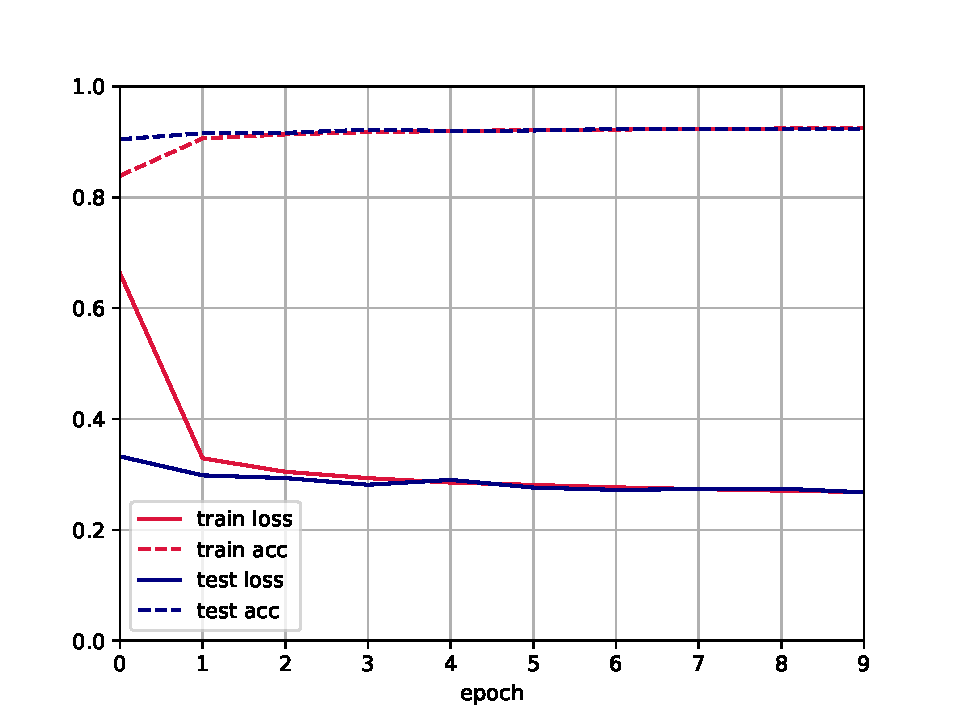
\includegraphics[width=\linewidth]{final_plot}

Code:

\begin{lstlisting}[language=Python]
n_inputs = 'not implemented'
n_hiddens = 'not implemented'
n_outputs = 'not implemented'

W1 = 'not implemented'
b1 = 'not implemented'
W2 = 'not implemented'
b2 = 'not implemented'



def relu(x):
    'not implemented'



def softmax(x):
    'not implemented'



def net(X):
  'not implemented'



def cross_entropy(y_hat, y):
  'not implemented'



def sgd(params, lr=0.1):
  'not implemented'



def train(net, params, train_iter, loss_func=cross_entropy, updater=sgd):
  'not implemented'

\end{lstlisting}

\newpage

%%%%%%%%%%%%%%%%%%%%%%%%%%%%%%%%%%%%%%%%%%%%%
% Problem 4
%%%%%%%%%%%%%%%%%%%%%%%%%%%%%%%%%%%%%%%%%%%%%

\begin{problem}[Impact Question: Testing security of neural networks deployed in autonomous vehicles and suggesting policy recommendations (9 points)]

\textbf{The learning goal of the impact questions of this homework is
three-fold: }

\begin{enumerate}
\item
  Get trained in adversarial thinking to be able to anticipate risks and
  possible exploits when designing Machine Learning applications
\item
  Understand opportunities and limitations to safety and security of
  Machine Learning applications
\item
  Learn to put yourself in the shoes of policymakers who are in charge
  of ensuring safety of real-world Machine Learning applications.
\end{enumerate}

\textbf{Prompt: }You are the Director of Machine Learning of the US
Department of Transportation (a federal US government agency).

The Secretary of the US Department of Transportation declares security
of Machine Learning applications deployed in autonomous vehicles as one
of the priorities of the agency. You are tasked to assess the security
of Machine Learning systems deployed in autonomous vehicles and develop
policy recommendations for the US Department of Transportation.

\textbf{Context: }Tesla employs Neural Networks for perception and
control tasks: For example semantic segmentation, object detection and
monocular depth estimation is performed by Neural Networks on images
captured with the car's camera system to identify road signs, traffic
lights, pedestrians, cars or other traffic related individuals,
vehicles, and objects. The full build autopilot consists of more than 48
networks which must identify high-risk scenarios and provide robust
predictions to ensure safety.

Moreover, beyond cameras Tesla also uses additional sensor systems such
as LiDAR or ultrasonic sensors. Yet, Tesla's engineering and design
approaches are still iterated and their software gets updated.

Link to a demo video: \url{https://tesla-cdn.thron.com/static/NGSLYL_network_XZCUMR.mp4}

Please answer the questions below by using concise language (350 - 700
words in total). Bullet points are appropriate.

\textbf{Questions: }

\begin{enumerate}
\item
  \textbf{Adversarial thinking: }List and explain 3 options how you
  could attack the Neural Network deployed in a self-driving car to make
  it crash. In particular, explain the impact of the attack on the
  statistical properties of input data and predictions of the Neural
  Network. (3 points)

  \begin{enumerate}
  \item
    \textbf{Hardware adversarial attack: }List and explain one attack
    which targets the hardware system of an autonomous vehicle or its
    physical surround.
  \item
    \textbf{Software adversarial attack:} List and explain one attack
    which targets the software system of an autonomous vehicle.
  \item
    \textbf{Social engineering:} List and explain one attack which
    relies on social engineering to make an autonomous vehicle crash.
  \end{enumerate}

\item
  \textbf{Safeguards: }For each of the 3 attack options that you listed
  above, suggest and explain one possible solution that could safeguard
  the Neural Network deployed in Tesla's autopilot. (3 points)

\item
  \textbf{Policy recommendation: }The Secretary of the US Department of
  Transportation asks you to develop one policy recommendation on how to
  ensure sufficient security of deployed neural networks in autonomous
  vehicles.

  \begin{enumerate}
  \item
    \textbf{Recommendation:} List and explain one policy recommendation
    that the US Department of Transportation should implement. (1 point)
  \item
    \textbf{Benefit: }List and explain one benefit of your chosen
    recommendation. (1 point)
  \item
    \textbf{Drawback: }List and explain one drawback of your chosen
    recommendation. (1 point)
  \end{enumerate}
\end{enumerate}

\end{problem}

\newpage

\subsection*{Solution:}


\newpage

%%%%%%%%%%%%%%%%%%%%%%%%%%%%%%%%%%%%%%%%%%%%%
% Name and Calibration
%%%%%%%%%%%%%%%%%%%%%%%%%%%%%%%%%%%%%%%%%%%%%
\subsection*{Name}

\subsection*{Collaborators and Resources}
Whom did you work with, and did you use any resources beyond cs181-textbook and your notes?

\subsection*{Calibration}
Approximately how long did this homework take you to complete (in hours)? 


\end{document}
